\chapter{项目介绍}

\section{项目目标}

本项目在于尝试特征提取算法,具体来说,本项目以人脸图像为例,就人脸图像的特征提取展开了讨论.主要分为两个部分.
\paragraph{基于全局的特征提取算法} 本文首先实现了PCA, NMF, ICA等全局特征提取算法,这些算法有压缩率大,运行效率较高的优点,但也有着无法辨别背景,识别率存在上限的缺点.在对这些特征提取算法比较之后,作者发现比较难以实现精确的人脸识别,于是便开始了基于局部的特征提取算法的探究.
\paragraph{基于局部的特征提取算法} 本文以SIFT算子为例,实现了局部的特征提取算法.并对SIFT算子进行了一定的优化.SIFT相比较PCA算子,具有能区分背景,基于图像变换最大,信息最多的地方描述的优点.但是,也同时发现了SIFT算法计算速度较慢,内存占用大的缺点.\newline


本文从以上两个角度来对人脸图像的特征提取算法进行了分类,并尝试通过模型比较的方法来为实际应用中的算法,参数选择提供参考.

\todo{Background Research}

\section{项目范围}
人脸识别是一个比较大的内容,它主要分为以下几个步骤:
\begin{enumerate}
	\item{基本的图像处理:} 这一部分把人脸图像做普通的图像处理,使用基本的图像处理算法,来进行如加深对比度,亮度平衡,去噪等操作.
	\item{人脸检测:} 由于很多情况下人脸并非实际应用图片中的唯一物体,大多数情况下需要使用算法在普通图片中识别出人脸来单独处理.
	\item{降维操作:}  由于人脸图像作为由灰度值或彩色值表示的矩阵,直接处理中存在着类内差别大,向量维数大,数据冗余度高等诸多缺点.需要将人脸图像的特征提取出来,并具体就其特征深入处理.
	\item{识别操作:} 提取出人脸的特征后,人脸识别问题就被转化为经典的机器学习问题了.可以把模型描述为"给定了人脸的特征向量,来恢复人脸标签"的监督或非监督机器学习问题.
\end{enumerate}

而本项目主要探究的话题在于问题3,也就是给定了人脸图像,从中提取更有表现力的特征向量的问题.从这个角度上,本文从多个角度,提取了多种特征向量,并结合了多种分类算法,来探究不同特征提取算法,及同一特征提取算法不同参数下的性能优劣.
\section{本项目报告的结构}
\begin{enumerate}
	\item 本报告第一章是关于项目的简单介绍
	\item 本报告第二章详细介绍了多种基于全局的特征提取算法
	\item 本报告第三章以SIFT算子为例,介绍了基于局部的特征提取算法
	\item 本报告第四章从多种角度(类间距离,结合分类机等)对前两章节实践的特征提取模型加以比较
\end{enumerate}
\section{用到的数据库}
本文用到了ORL数据库\cite{samaria1994parameterisation},ORL数据库由40人每人10张不同角度共计400张图片组成.

ORL数据库举例:
	
	\begin{center}
	\begin{minipage}[t]{\linewidth}
	%\label{fig:main}
	\center
	{
	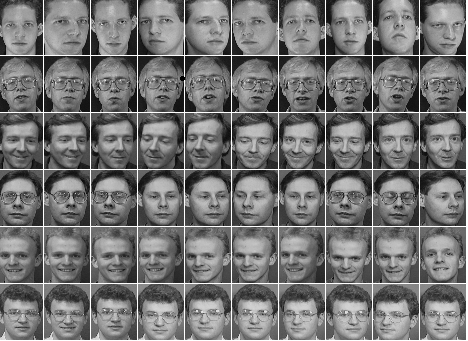
\includegraphics[width=\textwidth]{Img/faces} \captionof{figure}{ORL数据库举例}
	}
	\end{minipage}
	\medskip
	\end{center}
		
\section{项目应用}
值得一提的,本项目虽然是就人脸图片算法展开了讨论,但是实际应用并不仅限于此.在大多数处理过程中,人脸图片被展开并作为较长的向量处理,而之后对这个展开后向量的操作就可以被应用到其他高维数据的处理上去.本文中所讨论的算法可以有效的降维,减小数据冗余.\newline


其他可以应用高维处理算法的问题有:

\begin{itemize}
	\item{基因处理: } 基因是由A, T, C, G四种碱基组成序列,通常长度可以达到10-15k\cite{twine2011whole}.降维算法和特征提取算法可以更加有效地识别出基因的特征,从而帮助建立性状和基因的关系.
	\item{乐曲识别:} 乐曲可以被视作很长的电信号序列.在音乐幅值谱上的特征提取可以识别音乐的流派,歌手等信息.
\end{itemize}



\section{本项目内容及真实性声明}

本项目大部分代码都在\textit{Matlab 2015b}下运行,本报告由 \LaTeX 撰写. 同时项目及项目报告都使用了\textit{Git}来进行项目管理.主要内容有:
\begin{enumerate}
	\item \url{https://github.com/y1275963/Eigenfaces} 项目的主体内容,包括了基本代码的实现
	\item \url{https://github.com/y1275963/bachelor_thesis} 项目报告的主体内容,包括文章本身及文章中的插图
	\item \url{https://www.dropbox.com/sh/zlie193xdxog7i7/AACAmN5ddQE0-Fn9NgGLeSIsa?dl=0} 本地运行结果缓存, 由于很多情况下,本项目涉及了参数扫描的过程,这些过程运行时间比较长,因此为了方便绘图的缘故也对结果进行了缓存
\end{enumerate}

在项目报告的附录中,详细罗列了使用到的软件库及原始数据,同时也简略罗列了开发记录.\newline


作者在此声明,文章中所有出现的图片,表格均由作者本人亲自得到,并在项目报告中尽力详细描述了具体实现中的参数选择.